\documentclass{article}

\usepackage[utf8]{inputenc}
\usepackage{xcolor}
\usepackage{textcomp}
\usepackage[T1]{fontenc}
\usepackage{pdfpages}

\title{geschichte}
\author{marius cramer}
\date{17-08-2018}

\definecolor{myGreen}{RGB}{97, 154, 76}
\definecolor{myRed}{RGB}{176, 72, 72}
\definecolor{myBlue}{RGB}{77, 130, 185}
\definecolor{myOrange}{RGB}{221, 137, 51}

\setlength{\parindent}{1em}
\setlength{\parskip}{1em}

\begin{document}
\maketitle

\section{Lernbereiche}
\begin{enumerate}
  \item Europa auf dem Weg in die Moderne: Reform und Revolution
  \item Nation - Nationalismus - Nationale Identität
  \item Demokratie und Diktatur
  \item Europa- und Weltpolitik im Spannungsfeld von Interessen und Werten
\end{enumerate}

\section{Einführung}
Was ist und wozu betreiben wir Geschichte?

marius -\guilsinglright  Geschichte ist eine vergangene Zeit welche erinnerungswert für die Allgemeinheit ist. Sie wird betrieben um an guten sowie schlechten Erinnerungen festzuhalten.

ilse -\guilsinglright  Geschichte ist die uns bekannte Vergangenheit über Menschen und Natur. Sie kann zeigen das gegenwärtige Existenz aus Elementen der Vergangenheit besteht und durch sie bedingt ist.

\par

Ausarbeitung \textcolor{myGreen}{Schiller}, \textcolor{myRed}{Nietzsche} und \textcolor{myBlue}{Lenz}:
\textcolor{myRed}{Nietzsche}: Für Nietzsche gibt es 3 Arten der Historie, eine monumentalische, eine antiquarische und eine kritische. Die monumentalische Betrachtung der Vergangenheit dient dazu, den großen Überblick über die Geschichte zu erlangen, diese gibt dem Menschen Mut, da er versichert wird, dass etwas was in der Vergangenheit schon einmal passierte auch wieder passieren kann, im Guten sowie im Schlechten.
"Die antiquarische Historie entwartet selbst in dem Augenblicke, in dem das frische Leben der Gegenwart sie nicht mehr beseelt und begeistert."
Die kritische Historie ist der Teil, aus dem man lernen soll. Wenn man die "Vergangenheit kritisch betrachtet, dann greift man mit dem Messer an seine Wurzeln, dann schreitet man grausam über alle Pietäten hinweg."

\section{Quellen}
\begin{itemize}
  \item Bild- und Tonquellen
  \item mündliche Quellen (Zeitzeugen)
  \item schriftliche Quellen (Faksimile)
  \item Sachquellen (Denkmäler, Funde, Ausgrabungen)
\end{itemize}

\medskip

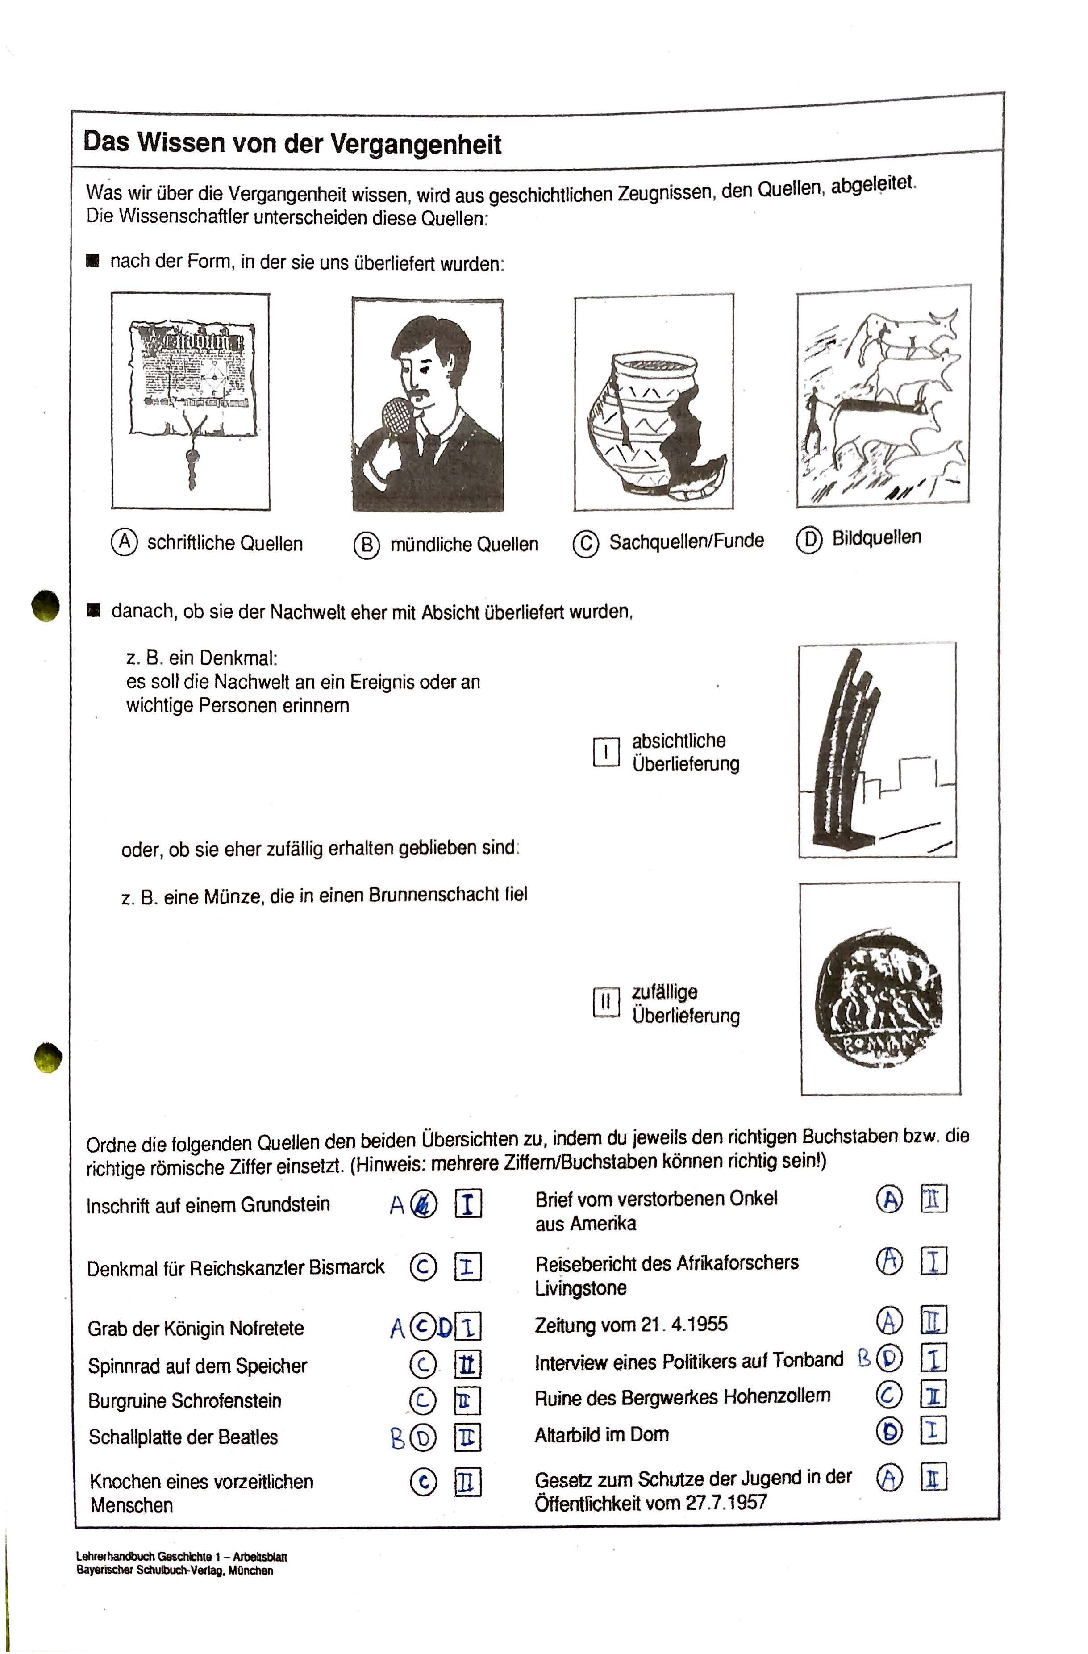
\includepdf[pages=-]{ges_wissen.pdf}
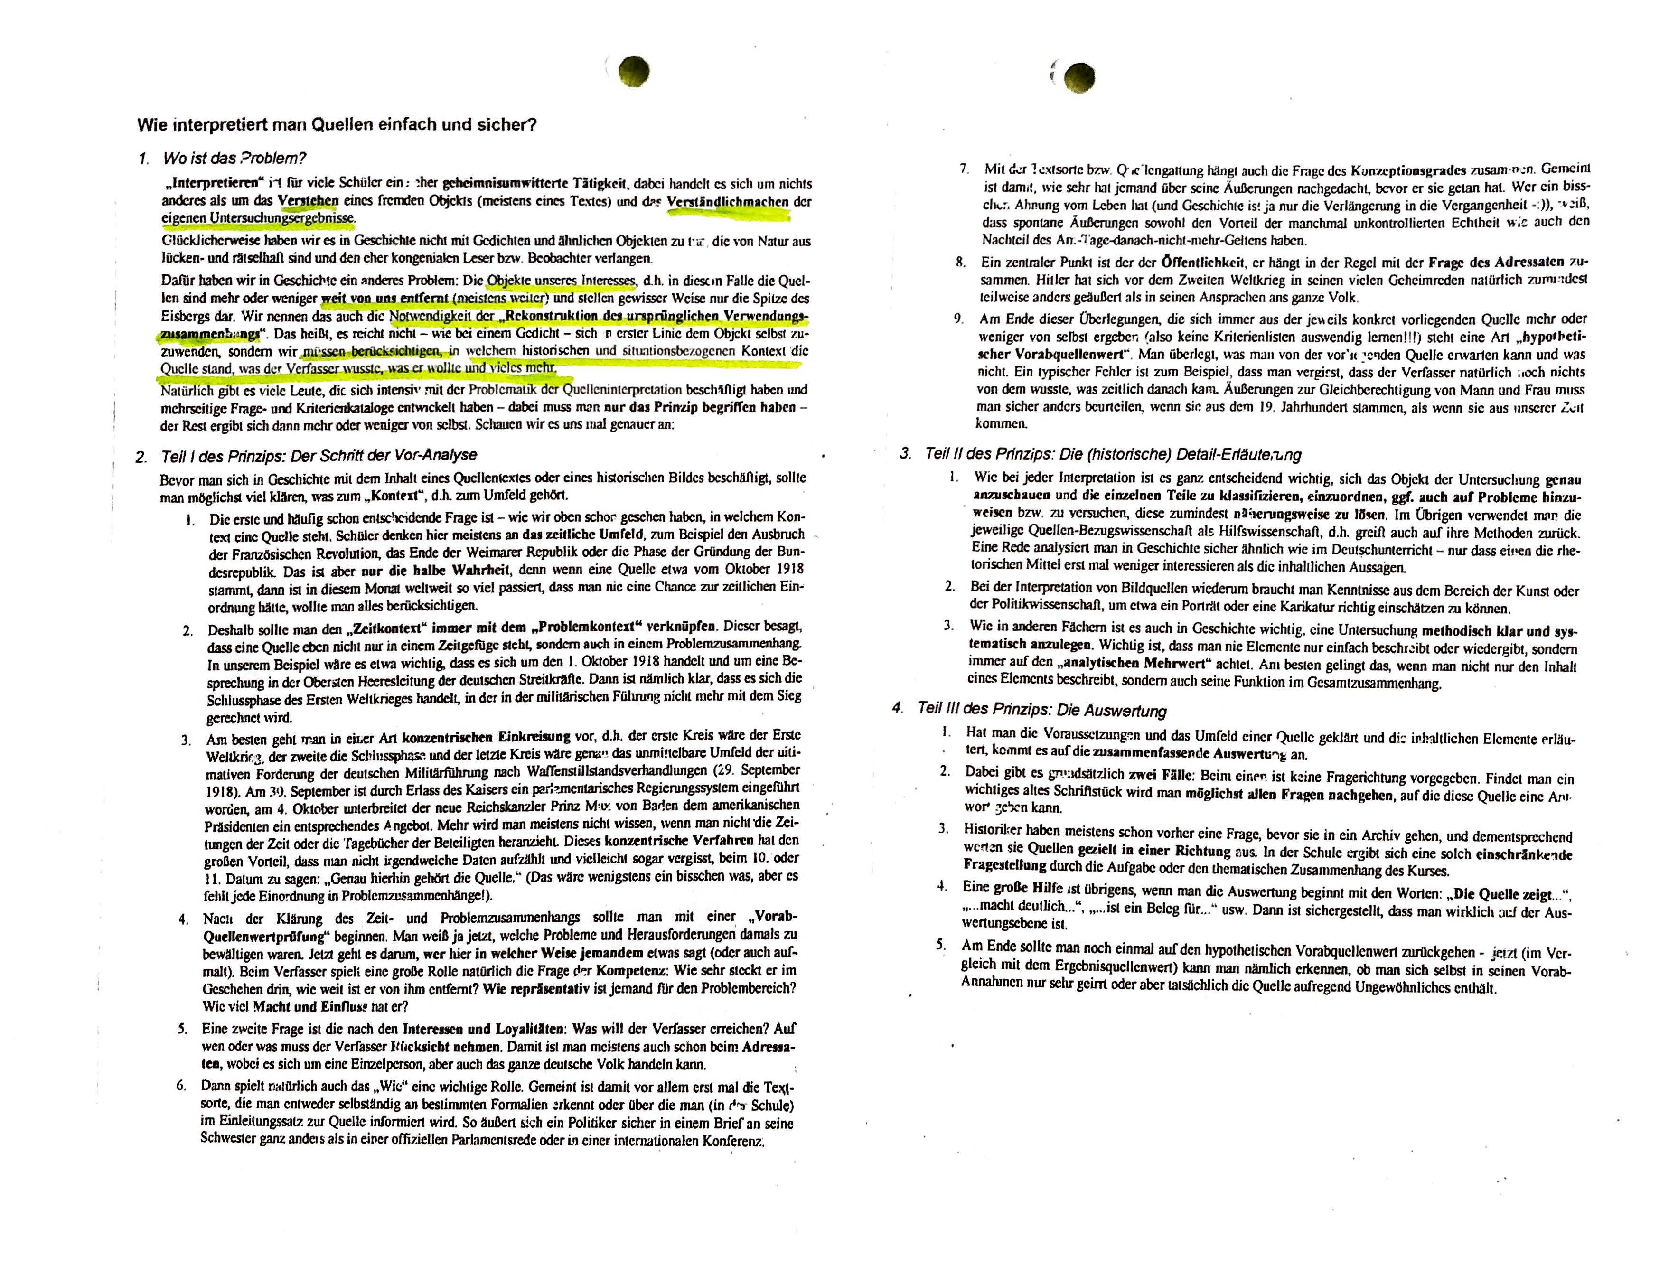
\includepdf[pages=-]{ges_quellen.pdf}

\section{Quelleninterpretation}
%\includepdf[pages=-]{ges_interpretation.pdf}

\begin{itemize}
  \item Original (Primärquelle) oder Übersetzung (Sekundärquelle)?
\end{itemize}

Bearbeitung eines Gesamttextes: Konzerpt + Erörterung
-Alle Informationen werden erfasst
Bearbeitung des Textes nach spezifischer Fragestellung: Exzerpt
-nur bestimmte, Fragestellungsrelevante Informationen werden erfasst

\subsection{Gliederung}
\begin{enumerate}
  \item Vorstellen der Quelle
  \item Übersichtssatz (Kerngedanke)
  \item Quellenbearbeitung
\end{enumerate}

\section{Aufgabe:}
\begin{enumerate}
  \item Analysiere die Quelle!
  \item Konspektiere sie!
  \item Exzerpiere! In welche Lager sieht der Verfasser die Demokraten gespalten?
\end{enumerate}

%\includepdf[pages=-]{ges_quelle01.pdf}

\textbf{Quellenkritische Analyse:}\newline
Verfasser: \textbf{Michael Geidel}\newline
Hintergrund: \textbf{Mauerfall und Vereinigung der DDR und BRD}\newline
Perspektive: \textbf{Die Quelle ist aus der Sicht von Michael Geidel geschrieben}\newline
Aussage der Quelle: \textbf{Die Quelle sagt aus, dass die Montagsdemonstrationen DDR immer aggressiver und unartiger werden. Geidel sagt: "Die Montagsdemonstrationen drohen zu entgleisen." Er fürchtet dies könnte zum Zusammenbruch der Sicherheit und Demokratie der DDR führen.}\newline
Struktur: \textbf{Die Quelle besteht aus zwei Teilen, im ersten erklärt Michael Geidel die momentane Situation, im zweiten schlägt er Lösungswege vor und wie man die gereizte Situation vermindern könnte.}\newline
Veröffentlichungsdatum: \textbf{05-12-2018}\newline
Örtliche/Zeitliche Hinweise: \textbf{keine}\newline
Bezüge: \textbf{Durch die zeitliche Einordnung der Situation weiß man das all dies vor dem Hitnergrund der Wiedervereinigung der DDR und BRD geschieht.}\newline
Präsentation: \textbf{Die Aussage wird in Textform übertragen.}\newline




\end{document}
